\documentclass{article}
% Template-specific packages
\usepackage[utf8]{inputenc} % Required for inputting international characters
\usepackage[T1]{fontenc} % Output font encoding for international characters
\usepackage{mathpazo} % Use the Palatino font

\usepackage{graphicx} % Required for including images

\usepackage{booktabs} % Required for better horizontal rules in tables

\usepackage{listings} % Required for insertion of code

\usepackage{enumerate} % To modify the enumerate environment
\usepackage{hyperref}
\usepackage{listings}
\lstset{
basicstyle=\small\ttfamily,
columns=flexible,
breaklines=true
}
\usepackage[utf8]{inputenc}
\usepackage{listings}

\lstset{
basicstyle=\small\ttfamily,
columns=flexible,
breaklines=true
}
\usepackage{fancyvrb}
\usepackage{enumitem}
\usepackage{graphicx}
\usepackage{geometry}
 \geometry{
 a4paper,
 total={6in , 10in},
 left=20mm,
 top=10mm,
 }
 
\usepackage{hyperref} 

\usepackage{graphicx}

\usepackage{listings}
\usepackage{enumitem}
\lstset{
basicstyle=\small\ttfamily,
columns=flexible,
breaklines=true
}

 
\title{Peter's Textbook on Database and SQL}
\author{TheProf.ca/ProfessorPeterSpeaks }
\date{October 2019}

\begin{document}
\maketitle
\tableofcontents

\newpage

\section{Database Design Project: DUE October 25  11:59 PM:}
\subsection{The CONCEPT:}

Your Team is going to create a fully functional Database in MS SQL SERVER that could be used to run a BUSINESS, or implement some business processes.
\subsection{Your Deliverables: A Latex Document and a Video}
\subsection{Project Grading Rubric}
\begin{enumerate}
    \item Quality of your Tracability Matrix and Test Cases: 25\%
    \item Quality of your SQL Statements and PROJECT SHOULD ACTUALLY WORK! (PASS ALL TEST CASES!:   25\%
    \item A Latex Document: 25\%   Contents:
    \item Charts, Diagrams (http://draw.io)    
    \item Write Descriptions  
    \item That explain how to produce your project  
    \item Examples of work product MUST include: SQL Statements, Business Process Descriptions presented with Use Cases and UML.
    \item A Video Posted on Youtube:  25\%
    \item Your Video is going to design and explain your PROJECT DESIGN to a technically knowledgeable young person who wants to reproduce your work.  
    \item You will work in Teams assigned by the Instructor.    
\end{enumerate}

\section{Tips and Suggestions on Making a Video Presentation:}

\begin{itemize}
    \item Speak to the CAMERA as if you were speaking to a student you were teaching this too
    \item Use Support Visuals, such as drawing on the White Board
    \item use you CELL PHONE to record the Video. Upload it to Youtube. Record the URL in your LATEX Document.
\end{itemize}

\newpage


\section{Week 06 Learning Agenda:}

\begin{itemize}
    \item SQL Design Project in class using Stored Procedures
    \item Using VIEWS as Tables 
    % https://www.udemy.com/course/sql-server-essentials-in-an-hour-the-select-statement/learn/lecture/8589804#overview
    \item Derived Columns
    \item Using the Index
    \item Backup and Restore of the Database
\end{itemize}    

% Done in Week 05. October 2 and 3

\section{SQL Design Project 10\%}

\subsubsection{See TEAM Assignments here:}
\url{https://drive.google.com/file/d/1LXf0c1oyE-j6egKsoXmYD6pn_quQor8e/view?usp=sharing}

\subsection{What you are to deliver:}


\begin{enumerate}
\item Use Draw.io to develop this together in Class: 
\item Here is your ARCHITECTURAL BLUEPRINT 
\item \url{https://drive.google.com/file/d/1Eo2B8aOWXoScFxXGSgrvW0yX29p9BKIe/view?usp=sharing}
\end{enumerate}

\vspace{.5cm}
Following the Procedures we have developed in class:
\begin{enumerate}
    \item Construct an SQL Statement to deliver one part of Jill's Trucking Company Database
    \item Post your SQL on the Classroom Server: 
    \url{https://www.dropbox.com/request/G4drfpdpDnfgNeWTB7X5}
    \item You can download other team's work product here: 
    \url{https://www.dropbox.com/sh/mpkudntvonaa08z/AAA5BDosF8FMeLdp_4fOS3bva?dl=0}
    \item Download all the other team's Stored Procedures
    \item Assemble all 7 Code Files into one SQL Statement. Run the SQL. Demonstrate the Final Product to the Instructor.
\end{enumerate}

%\subsection{Grading Rubric:}
\section{How to DESIGN and ARCHITECT an IT SYSTEM: Using Unified Process}

\subsection{Systems Development Using Unified Process and the n-tier Application}

\begin{enumerate}
    \item Unified Process
    \item User Stories
    \item User Interface Prototyping
    \item Requirement Documents
    \item Use Cases
    \item UML Diagrams
    \item Tracability Matrix
\end{enumerate}

\section{UP Learning Outcomes:}
\begin{enumerate}
    \item Understanding the Role and purpose of business modeling in the enterprise.
    \item Being cognizant of the types of goals and outcomes that the company's senior managers and leaders want from you as a process and data model designer.
    \item Unified process of software design (See: https://en.wikipedia.org/wiki/Unified_Process for more details.)
    \item Being able to describe the use of use cases and UML diagrams, and the importance of being able to elicit requirements from stakeholders.
    \item Having a sense of how program code and database structures are derived from UML diagrams. 
\end{enumerate}
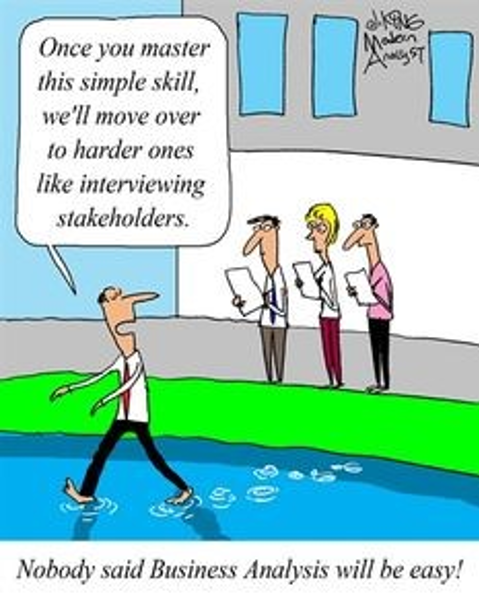
\includegraphics[scale=1.2]{Interviewing Stakeholders.png}
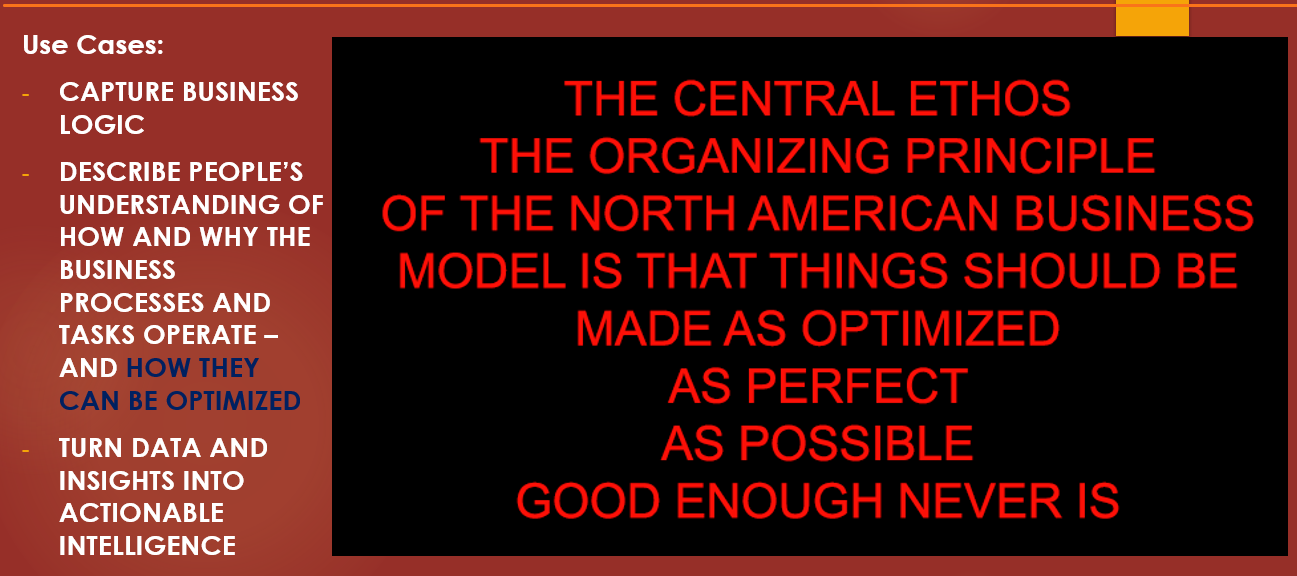
\includegraphics[scale=1.2]{use cases.png}


\subsection{Building the Tracability Matrix:}

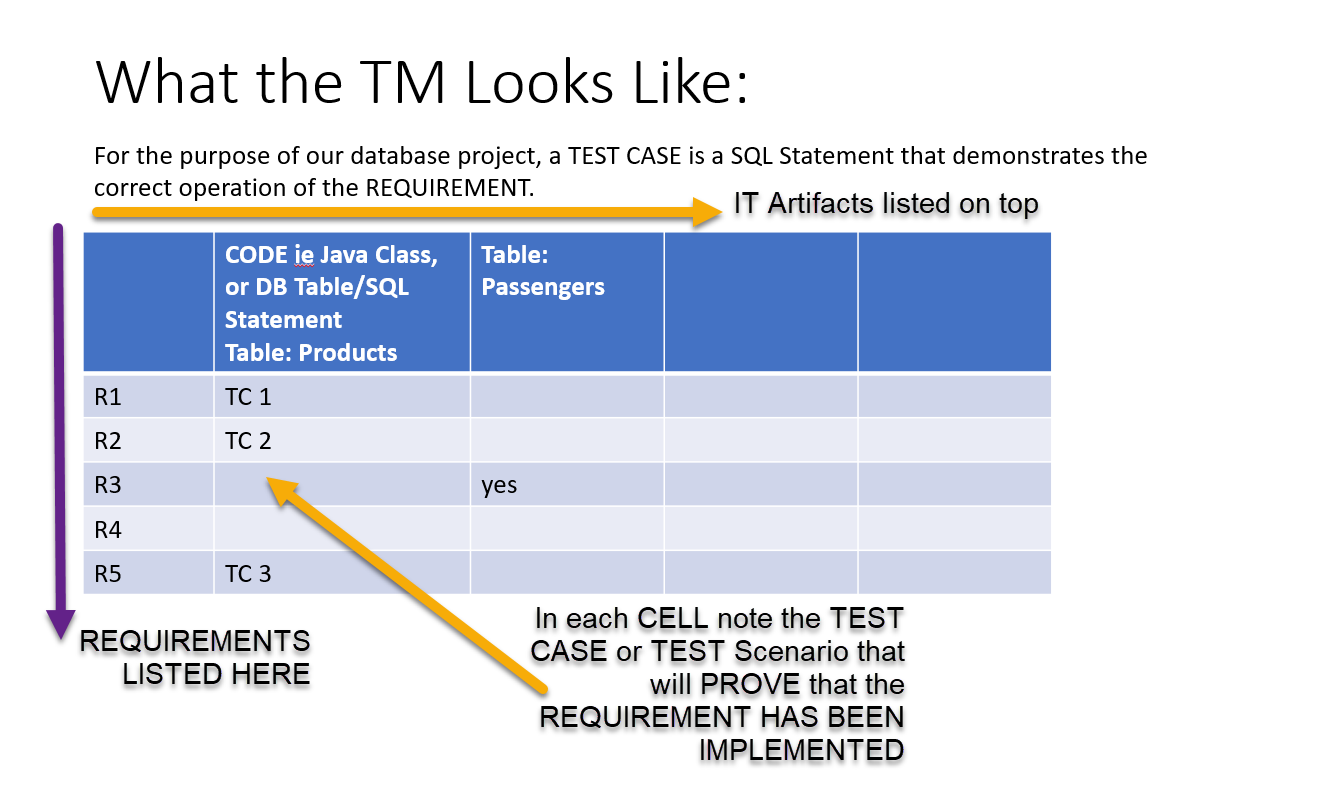
\includegraphics[scale=0.6]{images/TRACABILITYMATRIX.png}

\section{Requirements Analysis and Determination}

\begin{itemize}
    \item Writing a requirements document consists of interviewing stakeholders and user advocates. 
    \item A common practice is to ask them to write "user stories" - which just means that they will write down what ever they understand about how their job works.     
    \item Very few people really understand the details of the operation or job they're doing. The business analysts skill is to do the hard work of committing to diagrammatic communication (that's all UML diagrams are remember), and then sharing in joint application development sessions with the stakeholders and educating them until everyone can achieve a true consensus on what the system should do. 

    \item The Business Analyst may use UI Prototyping: Ask the users to draw out on paper Sketches of what the UI Screens should look with. The Screen is the User's Experience of the System.
    
\end{itemize}

The first and most critical skill for success as a business analyst is to commit to and work in a specific  industry domain, and apply yourself to becoming a subject management expert (SME).  

\newpage
\section {Creating and using Stored Procedures:}
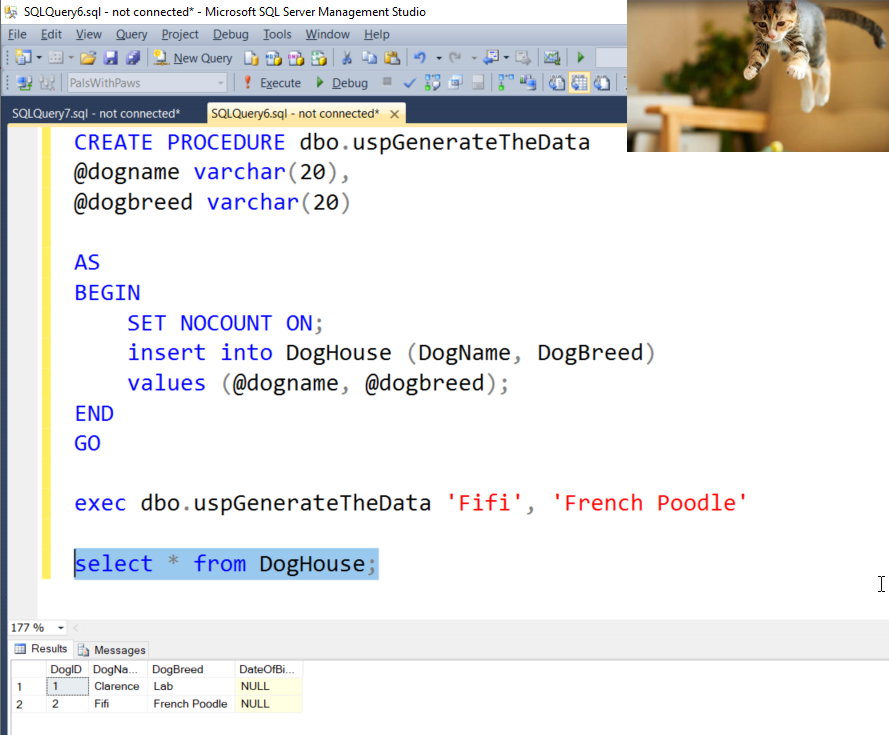
\includegraphics[scale=0.7]{images/RunningStoredProcedures.png}
\subsection {What is a Stored Procedure?}


\subsection{Why do we use Stored Procedures?}


\begin{itemize}
    \item S.P. can be called by outside program (eg JavaScript)
    \item S.P. can called by a a TRIGGER (which is just any condition in the database
    such as a certain table going above 1000 rows in number of records).
    \item Stored Procedures can provide a LIBRARY of Routines to make our development
    work speedier, less tiring, more efficient.
\end{itemize}

\subsection{How do we use Stored Procedures?}

\emph{Create a Stored Procedure:}
\begin{Verbatim}[frame=single]
create database PalsWithPaws;
GO

    CREATE PROCEDURE GenerateTheTables
    
    AS
    BEGIN
    	SET NOCOUNT ON;
    	create table DogHouse(
    		-- this is a comment
    		-- note how we set an AUTOINCREMENTING prmary key!
    		DogID int IDENTITY(1,1) PRIMARY KEY,
    		DogName varchar(20) not null,
    		DogBreed varchar(20) not null,
    		DateOfBirth datetime2 
    	);
    END
    GO
\end{Verbatim}

\emph{RUN a Stored Procedure:}
\begin{Verbatim}[frame=single]
exec GenerateTheTables
\end{Verbatim}

\section * {Parameterizing queries}
One of the benefits of SQL is the ability to write a query and use parameters to dynamically act upon the resultset. Depending on the situation, there can be benefits to parameterizing queries, but it is not always clear when or how to do this.  In this tip we look at different ways to pass in values as parameters to queries and the advantages and disadvantages.

\begin{Verbatim}[frame=single]

CREATE PROCEDURE dbo.uspGenerateTheData
@dogname varchar(20),
@dogbreed varchar(20)

AS
BEGIN
	SET NOCOUNT ON;
	insert into DogHouse (DogName, DogBreed) 
	values (@dogname, @dogbreed);
END
GO

\end{Verbatim}



\section {Week Learning Accomplishments}

\section  {Week 01}			

\begin{itemize}
\item Starting to learn what relational databases are. What is SQL? What is the Relational Database Model and how does it work?
\item Tables and Fields. Topics and Facts.
\item How does the relational database model compare with the Big Data Model?
\item What do Codd's Laws teach us? What did Codd's Laws do to advance the Cause of Civilization?
\item Primary Keys and Foreign Keys
\begin{itemize}
\item There are 6 Forms of Normalization.
\item Up to now, we have only talked about the First Normal Form: 1NF.
\item 1NF: Table A has a COLUMN with values that relate meaningfully to a COLUMN in Table B.
\item We create Predicate Joins by a few different methods. See the section: JOINING TABLES 
\item STUDY RESOURCE: \url{https://www.studytonight.com/dbms/database-normalization.php}
\end{itemize}

\begin{itemize}
\item The main reason for primary and foreign keys is to enforce data consistency.
\item A primary key enforces the consistency of uniqueness of values over one or more columns. If an ID column has a primary key then it is impossible to have two rows with the same ID value. Without that primary key, many rows could have the same ID value and you wouldn't be able to distinguish between them based on the ID value alone.
\item A foreign key enforces the consistency of data that points elsewhere. It ensures that the data which is pointed to actually exists. In a typical parent-child relationship, a foreign key ensures that every child always points at a parent and that the parent actually exists. Without the foreign key you could have "orphaned" children that point at a parent that doesn't exist.
\end{itemize}
\item Normalization and Minimization
\item 2 kinds of Informatics work: Analytics and Modeling
\item 4 kinds of SQL: Data Query Language, Data Manipulation Language, Data Control Language, Data Definition Language
\item Create Read Update Delete
\end{itemize}

\section {Week 02}
    
\begin{enumerate}
    \item Continuing the College Enrollment project
    \item Building up your Journal of SQL Statements in GitHub
     \item Using DDL to create Tables   
     \item Creating Scripts of SQL Statements   
     \item Using VIEWS
      \item Data Analytics : Creating Real Estate Market Reports
\end{enumerate}

\section {Week 03}
\subsection * {Farmer Joe SQL Exercise: Creating the Database and Writing the SQL}
\begin{enumerate}
    \item Data Definition Language: Creating the Tables
    \item Data Manipulation Language: Creating the Data
    \item Data Query Language
    \begin{itemize}
        \item Group By, Having, Aggregating Functions: Sum, Average, Max, Min 
        \item Using Views as Tables
        \item 4 kinds of joins: Left, Right, Inner, Outer
    \end{itemize} 
\end{enumerate}
    
\newpage
\section * {Week 04 Fill out Worksheet}
\textbf{}Week 04 Fill out Worksheet. \vspace{1cm} 
Name:   \vspace{1cm} 
Date:   \vspace{1cm} 
Class ID: \vspace{1cm}             \\
\begin{table}[]
\begin{tabular}{l|}
What does it mean to say that we do a PREDICATE JOIN on 2 SQL TABLES?  \vspace{1in}    \\

What are the differences between an INNER JOIN and a LEFT JOIN   \vspace{1in}       \\

What does an OUTER JOIN do?    \vspace{1in}      \\

How do we join tables using 1NF    \vspace{1in}     \\

Write a Query that uses a VIEW as a TABLE    \vspace{1in}     \\

Why do you LOVE 1NF ?  \vspace{1in}     \\

What are the most important elements of SQL and the Relational Database Model \\ as they relate to use as Data Modeling Specialists and Informatics Reporting Specialists? \\
For top marks, refer to Codd's Laws and 1NF    \vspace{3in}     \\

Discuss some of the principles of Information Systems Design that we have used in Class Exercises:   \vspace{3in}     \\



\end{tabular}
\end{table}

	
\iffalse

SQL Statements: Inner Joins

SQL Statements: Left Joins

SQL Statements: Right Joins

SQL Statements: Outer Joins

Creating Data Models: Joining Tables with Primary Keys and Predicate Joins

\fi 
\section{Samples and Patterns for Test Questions:}

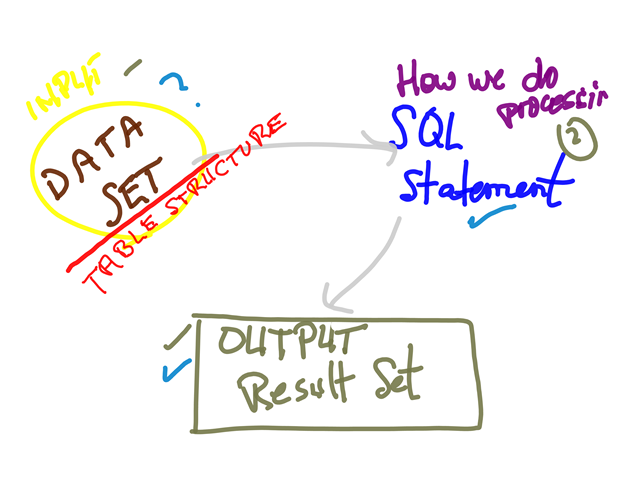
\includegraphics[]{images/dataset-sql-output.png}
\section{Joining Tables}

Predicate Joins are a sub set of CONDITIONS in SQL Clauses.

\subsection{Is there any difference (performance, best-practice, etc...) between putting a condition in the JOIN clause vs. the WHERE clause?}

\begin{verbatim}
    -- Condition in JOIN
SELECT *
FROM dbo.Customers AS CUS
INNER JOIN dbo.Orders AS ORD 
ON CUS.CustomerID = ORD.CustomerID
AND CUS.FirstName = 'John'

-- Condition in WHERE
SELECT *
FROM dbo.Customers AS CUS
INNER JOIN dbo.Orders AS ORD 
ON CUS.CustomerID = ORD.CustomerID
WHERE CUS.FirstName = 'John'

Which do you prefer (and perhaps why)?

\end{verbatim}
\newpage
\section {Principles of Information System Design}

\begin{verbatim}
First principle of Information Systems Design:
RESPONSIBILITY-DRIVEN DESIGN
Which PARTITION (database table or Java Class) is the best to :
1.	Store a piece of information
2.	To implement a certain business Process
TOPICS are the containers
FACTS are things that true in my environment which are relevant
\end{verbatim}

\section  * {SQL CONCEPTS}
	\subsection  * {Normalization}
	
	\begin{itemize}
	    \item We want many SMALL tables, not a few of BIG TABLES. This means can decouple our data sets.
	    \item Dr Codd - Cood's 13 Laws wants to RUN AWAY FROM the DATA FRAME in Cobol, in which all the data is scrunched together
	    \item NOW we need to connect TABLES together
	    \item connect tables on PK and FK if FIRST NORMAL Form

	\end{itemize}
		
\section {SQL Server}		
MS SQL Server is a HEADLess Application. Like an HTTP Server. You connect to it via a Client.		
			
\url{https://docs.microsoft.com/en-us/sql/linux/sql-server-linux-develop-use-vscode?view=sql-server-2017}	
\section  * {Farmer Joe}

\includegraphics[scale=0.6]{images/FarmerJoe.png}

\section{DDL to generate the Tables}
\begin{verbatim}
CREATE TABLE lots (
lot_id varchar(20),
quantity_of_vegatables int,
veggie_id varchar(20),
lot_name varchar(20),
PRIMARY KEY (lot_id)
);

CREATE TABLE veggies(
veggie_id varchar(20),
veggie_price money,
veggie_name varchar(20),
veggie_type varchar(20)
PRIMARY KEY (veggie_id)
);
\end{verbatim}


\section {Farmer Joe Exercise Data}

\begin{verbatim}
insert into veggies ( veggie_id, veggie_price, veggie_name, veggie_type  ) values ( '2' , 11, 'Peas', 'root' ) ;
insert into veggies ( veggie_id, veggie_price, veggie_name, veggie_type  ) values ( '3' , 8,  'Tomatos', 'root' ) ;
insert into veggies ( veggie_id, veggie_price, veggie_name, veggie_type  ) values ( '4' , 3,  'Corn', 'root' ) ;
insert into veggies ( veggie_id, veggie_price, veggie_name, veggie_type  ) values ( '5' , 3,  'Squash', 'root' ) ;
insert into veggies ( veggie_id, veggie_price, veggie_name, veggie_type  ) values ( '6' , 7,  'Artichokes', 'root' ) ;
insert into veggies ( veggie_id, veggie_price, veggie_name, veggie_type  ) values ( '6' , 9,  'Aubergines', 'root' ) ;
insert into veggies ( veggie_id, veggie_price, veggie_name, veggie_type  ) values ( '7' , 4,  'Asparagus', 'legumes' ) ;
insert into veggies ( veggie_id, veggie_price, veggie_name, veggie_type  ) values ( '8' , 2,  'Green bean', 'legumes' ) ;
insert into veggies ( veggie_id, veggie_price, veggie_name, veggie_type  ) values ( '9' , 8,  'Broccoflower', 'legumes') ;
insert into veggies ( veggie_id, veggie_price, veggie_name, veggie_type  ) values ( '10' , 12,  'Brussel Sprouts', 'legumes' ) ;
insert into veggies ( veggie_id, veggie_price, veggie_name, veggie_type  ) values ( '11' , 5,  'Brocelli', 'legumes' ) ;
insert into veggies ( veggie_id, veggie_price, veggie_name, veggie_type  ) values ( '12' , 6,  'Spinach', 'legumes') ;
\end{verbatim}

\begin{verbatim}
insert into lots ( lot_id, quantity_of_vegatables, lot_name, veggie_id ) values ( '1' , 800,  'red', '1' ) ; 
insert into lots ( lot_id, quantity_of_vegatables, lot_name, veggie_id ) values ( '2' , 500,  'orange', '2' ) ; 
insert into lots ( lot_id, quantity_of_vegatables, lot_name, veggie_id ) values ( '3' , 300,  'yellow', '3' ) ; 
insert into lots ( lot_id, quantity_of_vegatables, lot_name, veggie_id ) values ( '4' , 450,  'brown', '4' ) ; 
insert into lots ( lot_id, quantity_of_vegatables, lot_name, veggie_id ) values ( '5' , 800,  'green', '5' ) ; 
insert into lots ( lot_id, quantity_of_vegatables, lot_name, veggie_id ) values ( '6' , 800,  'violet', '6' ) ; 
insert into lots ( lot_id, quantity_of_vegatables, lot_name, veggie_id ) values ( '7' , 950,  'fuschia', '7' ) ; 
insert into lots ( lot_id, quantity_of_vegatables, lot_name, veggie_id ) values ( '8' , 820,  'purple', '8' ) ; 
insert into lots ( lot_id, quantity_of_vegatables, lot_name, veggie_id ) values ( '9' , 400,  'CHARTREUSE', '9' ) ; 
insert into lots ( lot_id, quantity_of_vegatables, lot_name, veggie_id ) values ( '10' , 500,  'grey', '10' ) ; 
insert into lots ( lot_id, quantity_of_vegatables, lot_name, veggie_id ) values ( '11' , 375,  'magenta', '11' ) ; 
insert into lots ( lot_id, quantity_of_vegatables, lot_name, veggie_id ) values ( '12' , 675,  'cyan', '20' ) ; 
\end{verbatim}

\begin{verbatim}
Challenge 4:
REPORT ON:
a.	TOTAL AMOUNT OF ALL VEGATABLES ON THE FARM, ALL LOTS
b.	LOT WITH MOST VEGATABLES
c.	LOT WITH LEAST VEGATABLES
d.	AVERAGE NUMBER OF VEGATABLES ACROSS ALL FIELDS.

select sum (l.quantity_of_vegatables * v.veggie_price) 

from lots as l, veggies as v

where l.veggie_id = v.veggie_id

\end{verbatim}
\newpage
\section {This is a collection of SQL we developed in class exercises}

\begin{lstlisting}
    INSERT INTO students ( studentid, studentlastname, studentfirstname, programgroupname ) VALUES ( 'A101', 'Smith', 'John', 'CPCT');
INSERT INTO students ( studentid, studentlastname, studentfirstname, programgroupname ) VALUES ( 'A102', 'Jones', 'Mike', 'CPCT');
INSERT INTO students ( studentid, studentlastname, studentfirstname, programgroupname ) VALUES ( 'A103', 'Smith', 'Susan', 'CPCT');
INSERT INTO students ( studentid, studentlastname, studentfirstname, programgroupname ) VALUES ( 'A104', 'Bichon', 'Peanut', 'CPCT');
INSERT INTO students ( studentid, studentlastname, studentfirstname, programgroupname ) VALUES ( 'A105', 'Smith', 'John', 'CPCT');
INSERT INTO students ( studentid, studentlastname, studentfirstname, programgroupname ) VALUES ( 'A106', 'Kirk', 'James', 'CPCT');
INSERT INTO students ( studentid, studentlastname, studentfirstname, programgroupname ) VALUES ( 'A107', 'Archer', 'Jonathan', 'CPCT');
INSERT INTO students ( studentid, studentlastname, studentfirstname, programgroupname ) VALUES ( 'A108', 'Janeway', 'Catherine', 'CPCT');
INSERT INTO students ( studentid, studentlastname, studentfirstname, programgroupname ) VALUES ( 'A109', 'Sisko', 'Benjamin', 'CPCT');
INSERT INTO students ( studentid, studentlastname, studentfirstname, programgroupname ) VALUES ( 'A110', 'Pike', 'Christopher', 'CPCT');
INSERT INTO students ( studentid, studentlastname, studentfirstname, programgroupname ) VALUES ( 'A111', 'Scott', 'Montgommery', 'CPCT');
INSERT INTO students ( studentid, studentlastname, studentfirstname, programgroupname ) VALUES ( 'A112', 'Riker', 'William', 'CPCT');


How to create the students table with DDL:
CREATE TABLE students(
studentid VARCHAR (20) NOT NULL,
studentlastname VARCHAR (20) NOT NULL,
studentfirstname VARCHAR (20) NOT NULL,
programgroupname VARCHAR (20) NOT NULL,
term VARCHAR (20) NOT NULL
PRIMARY KEY (studentid)
);

CREATE TABLE classes(
classid VARCHAR (20) NOT NULL,
roomid VARCHAR (20) NOT NULL,
datetimeid VARCHAR (20) NOT NULL,
coursename VARCHAR (20) NOT NULL
PRIMARY KEY (classid)
);

CREATE TABLE programgroup(
pgid VARCHAR (20) NOT NULL,
programgroupname VARCHAR(20) NOT NULL,
sectionnumber VARCHAR (20) NOT NULL,
classid VARCHAR (20) NOT NULL
PRIMARY KEY (pgid)
);

How to rename a COLUMN
USE CESVERSION2;
GO
EXEC sp_rename 'students.studentgroup' , 'programgroup';
GO


How to subtract the COUNTS of 2 Tables
DECLARE @ThisYearCount BIGINT,
        @LastYearCount BIGINT,
        @Difference  BIGINT

SELECT @ThisYearCount = COUNT(*) FROM ThisYear

SELECT @LastYearCount = COUNT(*) FROM LastYear

SET @Difference = @ThisYearCount - @LastYearCount

Print @Difference


How to delete a Column from a Table:

ALTER TABLE Customers
DROP COLUMN ContactName;


create view CombinedData as 

select this.Description, this.Type, this.bedroom , c.communityname, c.communitydata

from ThisYear as this, communityinfo as c 

where [sold price] < 600000 

and this.Community = c.communityname;

select * from CombinedData as cv where cv.bedroom  >3


WEEK 3 Code:

Farmer Joe Exercise:

CREATE TABLE veggies (
    veggie_id varchar(20),
    cost money,
    veggie_name varchar(20),
    quantity int
    PRIMARY KEY (veggie_id)
);

CREATE TABLE lot (
    lot_id varchar(20),
    veggie_id varchar(20),
    lot_name varchar(20),
    PRIMARY KEY (lot_id)
);




CREATE TABLE veggies(
veggie_id varchar(20),
veggie_price money,
veggie_name varchar(20),
veggie_type varchar(20)
PRIMARY KEY (veggie_id)
);

How to print out all fields in ALL Tables in a Database:

 SELECT TABLE_SCHEMA ,
       TABLE_NAME ,
       COLUMN_NAME ,
       ORDINAL_POSITION ,
       COLUMN_DEFAULT ,
       DATA_TYPE ,
       CHARACTER_MAXIMUM_LENGTH ,
       NUMERIC_PRECISION ,
       NUMERIC_PRECISION_RADIX ,
       NUMERIC_SCALE ,
       DATETIME_PRECISION
FROM   INFORMATION_SCHEMA.COLUMNS;


This example uses an expression and gives it a column alias.

SELECT
first_name,
last_name,
first_name || ' ' || last_name AS full_name
FROM employee_test;

This example uses a column alias on a function.

SELECT
last_name,
hdt AS hire_date,
ROUND(MONTHS_BETWEEN(SYSDATE, hdt),0) AS tenure_months
FROM employee_test;

\end{lstlisting}
\section * {SQL Commands}

\begin{verbatim}
  
SQL Statement	Syntax
AND / OR	SELECT column_name(s)
FROM table_name
WHERE condition
AND|OR condition
ALTER TABLE	ALTER TABLE table_name
ADD column_name datatype
or

ALTER TABLE table_name
DROP COLUMN column_name

AS (alias)	SELECT column_name AS column_alias
FROM table_name
or

SELECT column_name
FROM table_name  AS table_alias

BETWEEN	SELECT column_name(s)
FROM table_name
WHERE column_name
BETWEEN value1 AND value2
CREATE DATABASE	CREATE DATABASE database_name
CREATE TABLE	CREATE TABLE table_name
(
column_name1 data_type,
column_name2 data_type,
column_name3 data_type,
...
)
CREATE INDEX	CREATE INDEX index_name
ON table_name (column_name)
or

CREATE UNIQUE INDEX index_name
ON table_name (column_name)

CREATE VIEW	CREATE VIEW view_name AS
SELECT column_name(s)
FROM table_name
WHERE condition
DELETE	DELETE FROM table_name
WHERE some_column=some_value
or

DELETE FROM table_name
(Note: Deletes the entire table!!)

DELETE * FROM table_name
(Note: Deletes the entire table!!)

DROP DATABASE	DROP DATABASE database_name
DROP INDEX	DROP INDEX table_name.index_name (SQL Server)
DROP INDEX index_name ON table_name (MS Access)
DROP INDEX index_name (DB2/Oracle)
ALTER TABLE table_name
DROP INDEX index_name (MySQL)
DROP TABLE	DROP TABLE table_name
EXISTS	IF EXISTS (SELECT * FROM table_name WHERE id = ?)
BEGIN
--do what needs to be done if exists
END
ELSE
BEGIN
--do what needs to be done if not
END
GROUP BY	SELECT column_name, aggregate_function(column_name)
FROM table_name
WHERE column_name operator value
GROUP BY column_name
HAVING	SELECT column_name, aggregate_function(column_name)
FROM table_name
WHERE column_name operator value
GROUP BY column_name
HAVING aggregate_function(column_name) operator value
IN	SELECT column_name(s)
FROM table_name
WHERE column_name
IN (value1,value2,..)
INSERT INTO	INSERT INTO table_name
VALUES (value1, value2, value3,....)
or

INSERT INTO table_name
(column1, column2, column3,...)
VALUES (value1, value2, value3,....)

INNER JOIN	SELECT column_name(s)
FROM table_name1
INNER JOIN table_name2
ON table_name1.column_name=table_name2.column_name
LEFT JOIN	SELECT column_name(s)
FROM table_name1
LEFT JOIN table_name2
ON table_name1.column_name=table_name2.column_name
RIGHT JOIN	SELECT column_name(s)
FROM table_name1
RIGHT JOIN table_name2
ON table_name1.column_name=table_name2.column_name
FULL JOIN	SELECT column_name(s)
FROM table_name1
FULL JOIN table_name2
ON table_name1.column_name=table_name2.column_name
LIKE	SELECT column_name(s)
FROM table_name
WHERE column_name LIKE pattern
ORDER BY	SELECT column_name(s)
FROM table_name
ORDER BY column_name [ASC|DESC]
SELECT	SELECT column_name(s)
FROM table_name
SELECT *	SELECT *
FROM table_name
SELECT DISTINCT	SELECT DISTINCT column_name(s)
FROM table_name
SELECT INTO	SELECT *
INTO new_table_name [IN externaldatabase]
FROM old_table_name
or

SELECT column_name(s)
INTO new_table_name [IN externaldatabase]
FROM old_table_name

SELECT TOP	SELECT TOP number|percent column_name(s)
FROM table_name
TRUNCATE TABLE	TRUNCATE TABLE table_name
UNION	SELECT column_name(s) FROM table_name1
UNION
SELECT column_name(s) FROM table_name2
UNION ALL	SELECT column_name(s) FROM table_name1
UNION ALL
SELECT column_name(s) FROM table_name2
UPDATE	UPDATE table_name
SET column1=value, column2=value,...
WHERE some_column=some_value
WHERE	SELECT column_name(s)
FROM table_name
WHERE column_name operator value

 \end{verbatim}
\newpage
\section {Creating and using Stored Procedures:}
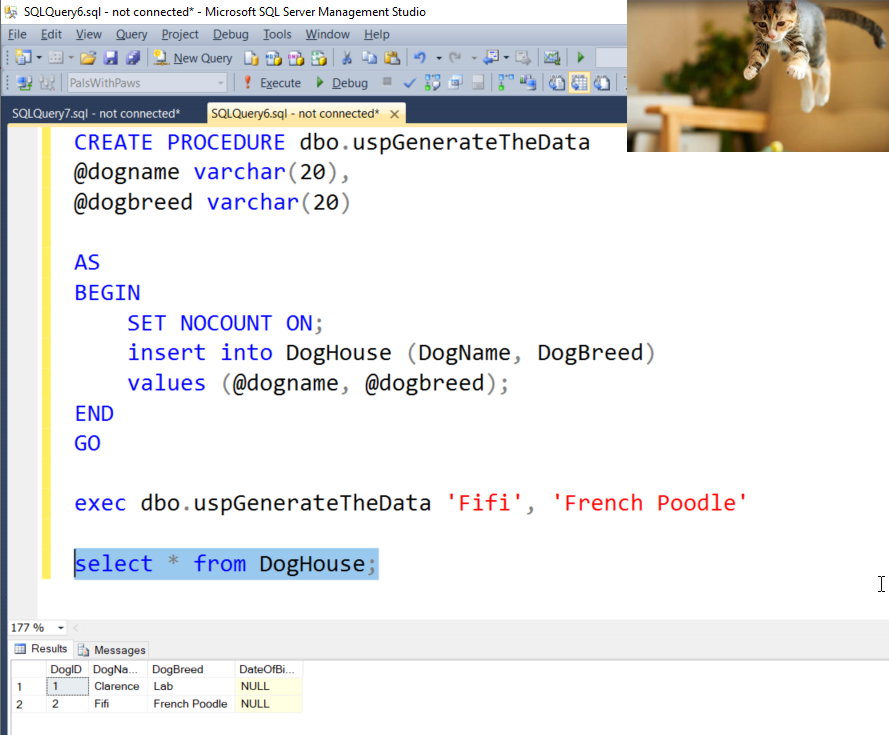
\includegraphics[scale=0.7]{images/RunningStoredProcedures.png}
\subsection {What is a Stored Procedure?}


\subsection{Why do we use Stored Procedures?}


\begin{itemize}
    \item S.P. can be called by outside program (eg JavaScript)
    \item S.P. can called by a a TRIGGER (which is just any condition in the database
    such as a certain table going above 1000 rows in number of records).
    \item Stored Procedures can provide a LIBRARY of Routines to make our development
    work speedier, less tiring, more efficient.
\end{itemize}

\subsection{How do we use Stored Procedures?}

\emph{Create a Stored Procedure:}
\begin{Verbatim}[frame=single]
create database PalsWithPaws;
GO

    CREATE PROCEDURE GenerateTheTables
    
    AS
    BEGIN
    	SET NOCOUNT ON;
    	create table DogHouse(
    		-- this is a comment
    		-- note how we set an AUTOINCREMENTING prmary key!
    		DogID int IDENTITY(1,1) PRIMARY KEY,
    		DogName varchar(20) not null,
    		DogBreed varchar(20) not null,
    		DateOfBirth datetime2 
    	);
    END
    GO
\end{Verbatim}

\emph{RUN a Stored Procedure:}
\begin{Verbatim}[frame=single]
exec GenerateTheTables
\end{Verbatim}

\section * {Parameterizing queries}
One of the benefits of SQL is the ability to write a query and use parameters to dynamically act upon the resultset. Depending on the situation, there can be benefits to parameterizing queries, but it is not always clear when or how to do this.  In this tip we look at different ways to pass in values as parameters to queries and the advantages and disadvantages.

\begin{Verbatim}[frame=single]

CREATE PROCEDURE dbo.uspGenerateTheData
@dogname varchar(20),
@dogbreed varchar(20)

AS
BEGIN
	SET NOCOUNT ON;
	insert into DogHouse (DogName, DogBreed) 
	values (@dogname, @dogbreed);
END
GO

\end{Verbatim}



\newpage
\section {SQL Programming Formulations}

\sample SQL Code using LATEX verbbatim:

\begin{verbatim}
    -- The following query can be used to sum the stock yet to be picked for all stock items.

DECLARE @StartingTime datetime2(7) = SYSDATETIME();

SELECT ol.StockItemID, [Description], SUM(Quantity - PickedQuantity) AS AllocatedQuantity
FROM Sales.OrderLines AS ol WITH (NOLOCK)
\end{verbatim}

\section {Using the PRINT command}
\begin{lstlisting}[frame=single]
PRINT 'Hello World';
DECLARE @myvariable VARCHAR(40) = 'I like essentialSQL.'
PRINT @myvariable
DECLARE @row INT = 63;
PRINT 'The value of row is ' + CAST(@row as VARCHAR);
\end{lstlisting}

\begin{lstlisting}[frame=single]

How to Use IF...THEN Logic in SQL Server

SQL Server has a unique capability of allowing you to execute real-time programmatic logic on the values within your query. Based on those logical evaluations, you can generate various values as part of the returned data set.

Using the CASE Statement
This is most easily accomplished in all versions of SQL Server using the CASE statement, which acts as a logical IF...THEN...ELSE expression and returns various values depending on the result.

In this example below, we want to return an additional locale column that specifies whether our book takes place in Middle-earth or regular old Earth.

SELECT
  CASE
    WHEN
      books.title = 'The Hobbit'
        THEN
          'Middle-earth'
    WHEN
      books.primary_author = 'Tolkien'
        THEN
          'Middle-earth'
    ELSE
      'Earth'
  END AS locale,
  books.*
FROM
  books
Before we examine the special CASE aspect of this statement, let’s temporarily remove the CASE to notice that this is an extremely simple SELECT statement on the surface:

SELECT
  books.*
FROM
  books
Therefore, let’s examine how the CASE section is structured and what logical behavior we’re performing.

CASE
  WHEN
    books.title = 'The Hobbit'
      THEN
        'Middle-earth'
  WHEN
    books.primary_author = 'Tolkien'
      THEN
        'Middle-earth'
  ELSE
    'Earth'
END AS locale
To begin, we of initialize the CASE statement then specify under which conditions (WHEN) our CASE statement should evaluate a result. In this example, we’re examining the books.title and books.primary_author; if either fit our Tolkien-esque theme, THEN we return the value ‘Middle-earth.’ If neither fields match our search, we instead return the value of ‘Earth.’

To rearrange the logic as a psuedo-code IF...THEN...ELSE statement, we’re simply asking SQL to evaluate:

IF
  title == 'The Hobbit' OR
  primary_author == 'Tolkien'
THEN
  RETURN 'Middle-earth'
ELSE
  RETURN 'Earth'
END
Finally, it is critical to remember that a CASE statement must always be appended at the end with a matching END statement. In the above example, we’re also renaming the resulting value that is returned to locale, though that is certainly optional.

Using the IIF Function
If you are using a more modern version of SQL, it is useful to know that SQL Server 2012 introduced the very handy IIF function. IIF is a shorthand method for performing an IF...ELSE/CASE statement and returning one of two values, depending on the evaluation of the result.

Restructuring our above example to use IIF is quite simple.

SELECT
  IIF(
    books.title = 'The Hobbit' OR books.primary_author = 'Tolkien',
    'Middle-earth',
    'Earth')
  AS locale,
  books.*
FROM
  books
With an IIF function, we largely replace a lot of the syntactical sugar from the CASE statement with a few simple comma-seperators to differentiate our arguments.

Both CASE and IIF get the same job done, but if given the choice, IIF will generally be much simpler to use.

\end{lstlisting}

\newpage

\begin{lstlisting}[frame=single]

SQL Server: FOR LOOP
Learn how to simulate the FOR LOOP in SQL Server (Transact-SQL) with syntax and examples.

TIP: Since the FOR LOOP does not exist in SQL Server, this page describes how to simulate a FOR LOOP using a WHILE LOOP.
Description
In SQL Server, there is no FOR LOOP. However, you simulate the FOR LOOP using the WHILE LOOP.

Syntax
The syntax to simulate the FOR Loop in SQL Server (Transact-SQL) is:

DECLARE @cnt INT = 0;

WHILE @cnt < cnt_total
BEGIN
   {...statements...}
   SET @cnt = @cnt + 1;
END;
Parameters or Arguments
cnt_total
The number of times that you want the simulated FOR LOOP (ie: WHILE LOOP) to execute.
statements
The statements of code to execute each pass through the loop.
Note
You can simulate the FOR LOOP in SQL Server (Transact-SQL) using the WHILE LOOP.
Example
Let's look at an example that shows how to simulate the FOR LOOP in SQL Server (Transact-SQL) using the WHILE LOOP.

For example:

DECLARE @cnt INT = 0;

WHILE @cnt < 10
BEGIN
   PRINT 'Inside simulated FOR LOOP on TechOnTheNet.com';
   SET @cnt = @cnt + 1;
END;

PRINT 'Done simulated FOR LOOP on TechOnTheNet.com';
GO
In this WHILE LOOP example, the loop would terminate once @cnt reaches 10.


\end{lstlisting}    
\newpage
\section  {Interesting places: Database and Programming Websites}

\begin{itemize}
\item \url{http://w3schools.com}
\item \url{http://sqlzoo.net} 
\item \url{http://repl.it} 
\subitem [online sql database to practice sql with]
\item ULTIMATE LIST OF 40 IMPORTANT SQL QUERIES 
\subitem \url{https://bytescout.com/blog/20-important-sql-queries.html}
\item SELECT Examples (Transact-SQL) 

\subitem \url{https://docs.microsoft.com/en-us/sql/t-sql/queries/select-examples-transact-sql?view=sql-server-2017}

\item \url{https://www.tsql.info/}
\item \url{http://www.sqlservertutorial.net/sql-server-basics/sql-server-update-join/}
\item \url{https://www.tutorialspoint.com/dbms}
\item \url{http://sqlfiddle.com}
\item \url{https://www.mytecbits.com/}
\item \url{https://www.tutorialgateway.org/}

SQL Server Tutorial https://www.tutorialgateway.org/sql/

\end{itemize}

\section  * {Lynda.com courses}
\url{https://www.lynda.com/SQL-tutorials/Welcome/529631/551694-4.html}

\url{http://openclassroom.stanford.edu/MainFolder/CoursePage.php?course=IntroToDatabases}


You can't use a variable for table name in the insert. You have to build that query dynamically too
https://stackoverflow.com/questions/29544132/msg-1087-level-16-state-1-line-25-must-declare-the-table-variable
\newpage
\section{TEST 1}
% \documentclass{exam}
% % Template-specific packages
\usepackage[utf8]{inputenc} % Required for inputting international characters
\usepackage[T1]{fontenc} % Output font encoding for international characters
\usepackage{mathpazo} % Use the Palatino font

\usepackage{graphicx} % Required for including images

\usepackage{booktabs} % Required for better horizontal rules in tables

\usepackage{listings} % Required for insertion of code

\usepackage{enumerate} % To modify the enumerate environment
\usepackage{hyperref}
\usepackage{listings}
\lstset{
basicstyle=\small\ttfamily,
columns=flexible,
breaklines=true
}
\usepackage[utf8]{inputenc}
\usepackage{listings}

\lstset{
basicstyle=\small\ttfamily,
columns=flexible,
breaklines=true
}
\usepackage{fancyvrb}
\usepackage{enumitem}
\usepackage{graphicx}
\usepackage{geometry}
 \geometry{
 a4paper,
 total={6in , 10in},
 left=20mm,
 top=10mm,
 }
 
\usepackage{hyperref} 

\usepackage{graphicx}

\usepackage{listings}
\usepackage{enumitem}
\lstset{
basicstyle=\small\ttfamily,
columns=flexible,
breaklines=true
}

%\begin{document}
 
\begin{center}
\fbox{\fbox{\parbox{5.5in}{\centering
CSD2206 Section ONE Test 1   5\% of final grade:
Total 70 Marks}}}
\end{center}
 
\makebox[\textwidth]{\enspace\ }
\vspace{2cm}
\makebox[\textwidth]{Name and Student ID:\enspace\hrulefill}

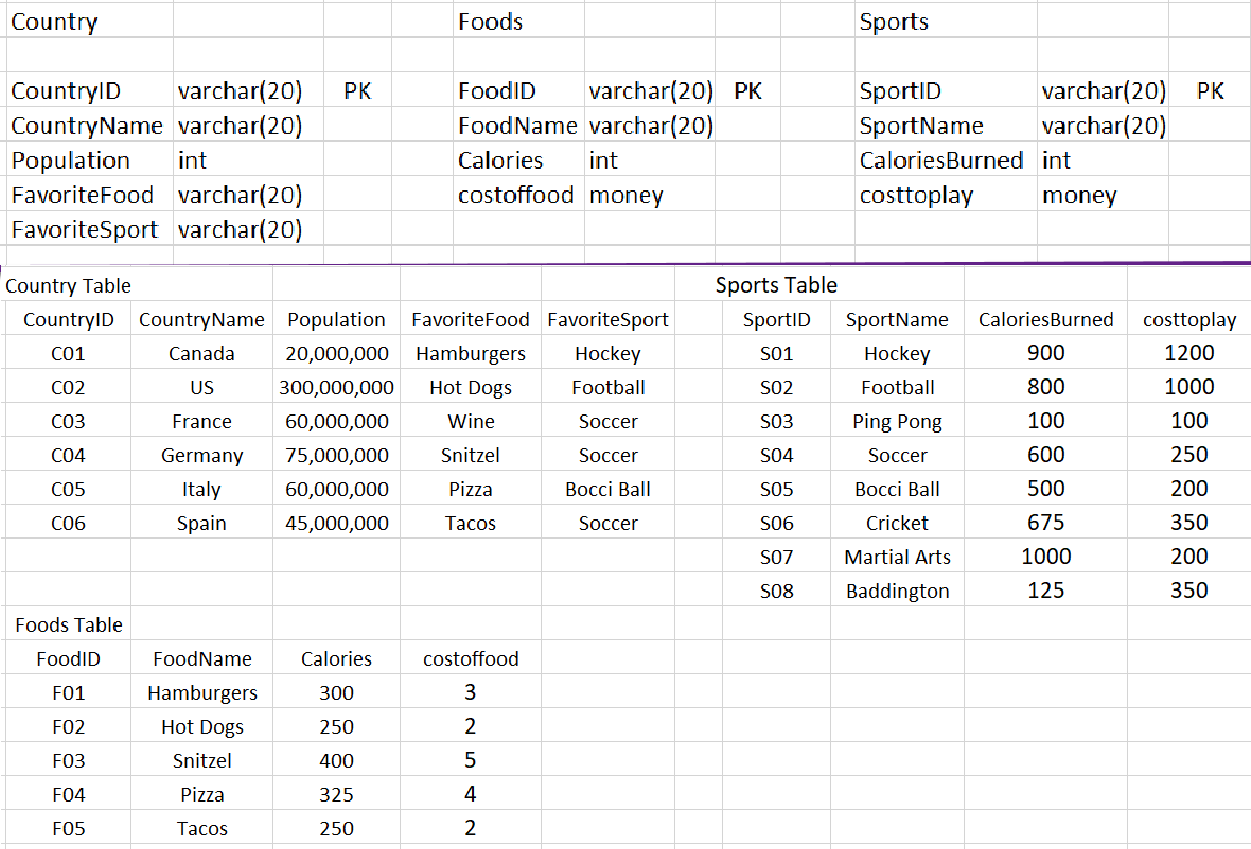
\includegraphics[scale=.5]{images/CountriesDatabaseImage.png}
\newline

\begin{questions}

\question 10 Marks: Write a SQL Statement to print out the SUM of all the 
calories BURNED by all the Sports Players in ALL COUNTRIES.
\vspace{4cm}

\question 10 Marks: Write a SQL Statement to print out the FAVORITE FOODS ORGANIZED BY FAVORITE SPORT:
\vspace{4cm}

\question 10 Marks: Write a VIEW to display much money is spent PER COUNTRY on Sports:
\vspace{4cm}

\question 10 Marks: Write a SQL Statement to create a new Country Table Record for Australia. For the values, make up some values that you think are probably correct:
\vspace{4cm}

\question 10 Marks: Write a SQL statement to print out a THE COST OF FOODS of the countries whose sports burn MORE THAN 600 calories:
\vspace{4cm}


\question 5 Marks: What is a ROWSET?
\vspace{4cm}

\question 5 Marks: What are the key features of the RELATIONAL DATABASE MODEL? When would it NOT be applicable?
\vspace{5cm}

\question 5 Marks: Why do you LOVE 1NF ?
\vspace{4cm}


\question 5 Marks: Describe Stored Procedures - What are they? Why do we use them? How do we use them?
\vspace{3cm}



\end{questions}

\end{document}


\end{document}